% % \section{Introduction}
% % \label{sec:introduction}

% % Relational databases support predictive decisions in commerce, finance, science, and online platforms. The evidence for one prediction is rarely contained in one row: customer churn may depend on transactions and products, while a race outcome may depend on drivers, constructors, and earlier results; in both cases, only information available before the prediction time may be used. Relational Deep Learning (RDL) represents rows as nodes and primary--foreign key (PK--FK) references as edges, replacing hand-engineered join-and-aggregate pipelines with learned relational models \citep{fey2024rdl}.  RelBench makes such temporal entity-prediction problems reproducible across real databases \citep{robinson2024relbench}.  Yet a new database or prediction target still commonly starts another supervised cycle: collect labels, optimize and validate a schema-specific model, and maintain a new deployment.  Reusing one model across databases would amortize this cost and enable prediction when target labels, compute, or deployment time are limited.

% % Cross-database transfer must balance relation specificity with schema variation. Table names and PK--FK identities are local to each database, although the structural roles they express often recur.  Consider Formula~1: both 
% % \texttt{Results}$\rightarrow$\texttt{Drivers} and 
% % \texttt{Results}$\rightarrow$\texttt{Races} are child-to-parent links, but one connects an outcome to who produced it and the other to the event in which it occurred (Figure~\ref{fig:architecture}).  Without relation-specific representations, a schema-independent row GNN cannot explicitly distinguish the roles of different database relations.  Assigning a learned embedding to every relation restores this specificity, but binds the model to the training schema and leaves relations in an unseen schema undefined.  Cross-database transfer therefore requires a third option: construct relation-specific representations on a new schema without binding model parameters to its relation identities.

% % Existing approaches make different choices in this tradeoff.  Row-based RDL models such as RelGNN~\citep{chen2025relgnn}, RelGT~\citep{dwivedi2026relgt}, and Griffin~\citep{wang2025griffin} preserve
% % explicit database structure and support compact structural computation, but their principal downstream protocols optimize parameters for the target task. Recent cross-database and relational in-context approaches instead reuse parameters across schemas through cell-token representations in RT~\citep{ranjan2026rt}, synthetic schema variation in
% % PluRel~\citep{kothapalli2026plurel}, column-preserving encoding in
% % RDBLearn~\citep{xu2026rdblearn}, or hierarchical row and column representations
% % in KumoRFM-2~\citep{hudovernik2026kumorfm2}.  These systems demonstrate reusable
% % prediction across databases while making different choices about representation granularity and contextual label access.  These alternatives motivate a compact row-level design that constructs relation-specific
% % representations for the current schema using parameters shared across databases.

% % \begin{figure*}[t]
% %   \centering
% %   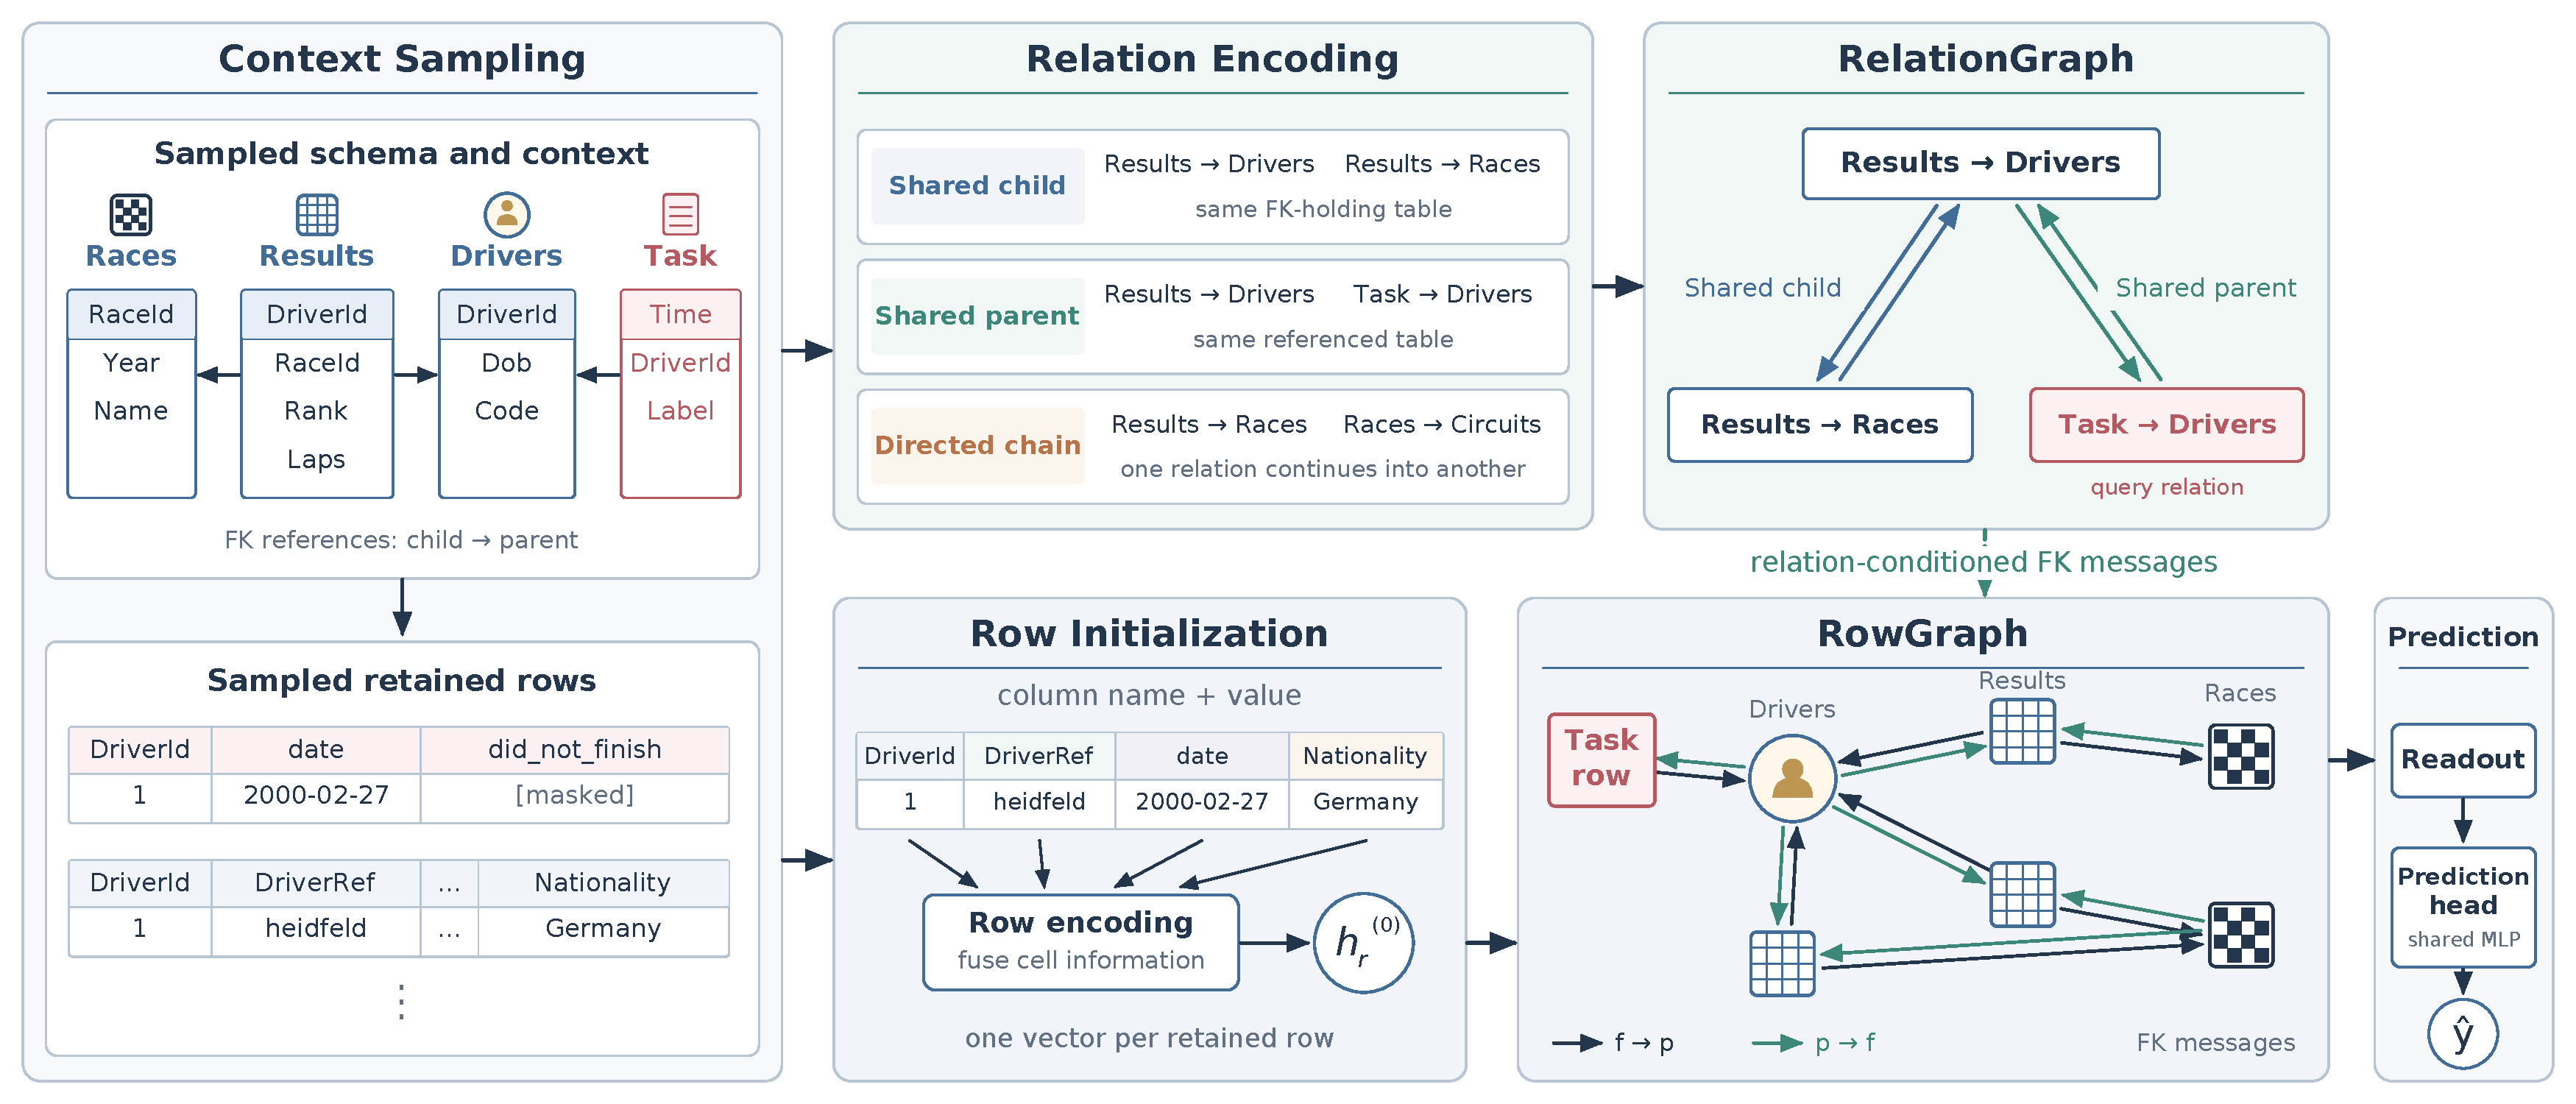
\includegraphics[width=\textwidth]{figures/architecture.pdf}
% %   \caption{High-level overview of \model{}.  A bounded temporal context is
% %   sampled, and visible heterogeneous cells are pooled once into row states.
% %   The retained PK--FK links instantiate two coupled graphs: an instance-level
% %   bidirectional row graph and a query-conditioned relation graph over ordered
% %   child--parent table pairs.  The relation states condition the corresponding
% %   foreign-to-primary ($\fkp$) and primary-to-foreign ($\pkf$) row messages,
% %   after which a shared candidate scorer, abstracted by the MLP block, produces
% %   the prediction.  Candidate nodes and label edges are omitted for clarity;
% %   red marks the query table, row, and seeded relation.}
% %   \label{fig:architecture}
% % \end{figure*}

% % We introduce \model{}, a compact row-level architecture for binary temporal entity classification on held-out relational databases (Figure~\ref{fig:architecture}).  Its context module samples a bounded, temporally valid neighborhood and aggregates visible heterogeneous cells into one representation per row.  Its relation-guidance module constructs a query-conditioned relation graph from the local PK--FK structure and uses shared structural interactions to infer relation representations without learned schema-specific identifiers.  Its row-reasoning module uses these representations to guide bidirectional message passing over the row graph, followed by a shared entity-classification readout.

% % Our contributions are:
% % \begin{itemize}
% %   \item We develop a compact row-graph architecture that combines bounded temporal context construction, heterogeneous row encoding, relation-guided message passing, and a shared entity-classification readout.
% %   \item We construct query-specific relation representations from schema-local structural interactions rather than learned table or relation identifiers, allowing the same operators to be applied to held-out database schemas.
% %   \item We evaluate \model{} on ten binary RelBench tasks under leave-database-out transfer.  It achieves 69.7 macro AUROC with 2.78M trainable parameters, and removing relation guidance reduces the score to 67.6.  A controlled target-history-masking evaluation further measures how strongly predictions depend on the query entity's previous labels.
% % \end{itemize}

% \section{Introduction}
% \label{sec:introduction}

% Relational databases support predictive decisions in commerce, finance,
% science, and online platforms. Evidence for these predictions is often
% distributed across interconnected tables, requiring models to combine
% information about an entity with its associated records. RelBench makes
% these problems accessible to systematic study by providing real-world
% relational databases, predictive tasks, and standardized temporal splits
% \citep{robinson2024relbench}. Relational Deep Learning (RDL) addresses such
% tasks by learning to aggregate information along primary--foreign key
% (PK--FK) connections, reducing the need for manually designed joins and
% feature aggregation \citep{fey2024rdl}. However, in the common task-specific
% supervised setting, a new database or prediction target requires another
% cycle of model training and validation. Reusing a unified model across
% databases would reduce this repeated effort and support prediction when
% target-task training resources are limited.

% Recent relational foundation models have demonstrated the feasibility of
% cross-database prediction \citep{ranjan2026rt}. A central design challenge is
% to preserve relation-specific computation while sharing parameters across
% different schemas. Consider Formula~1: both
% \texttt{Results}$\rightarrow$\texttt{Drivers} and
% \texttt{Results}$\rightarrow$\texttt{Races} are child-to-parent connections,
% but one associates a result with a driver, whereas the other places it
% within a race. Their shared direction alone does not capture these different
% roles in connecting predictive evidence. Representing relations beyond their
% FK direction allows the model to explicitly condition information
% propagation on the connections involved. Across databases, however, table
% identities and relation vocabularies change, making it necessary to construct
% such representations without relying on a fixed set of learned relation
% embeddings. Inspired by ULTRA \citep{galkin2024ultra}, we construct a
% query-conditioned RelationGraph whose nodes represent ordered child--parent
% table pairs. Shared operators encode their structural interactions to
% generate relation representations that can be applied to unseen schemas.

% \begin{figure*}[t]
%   \centering
%   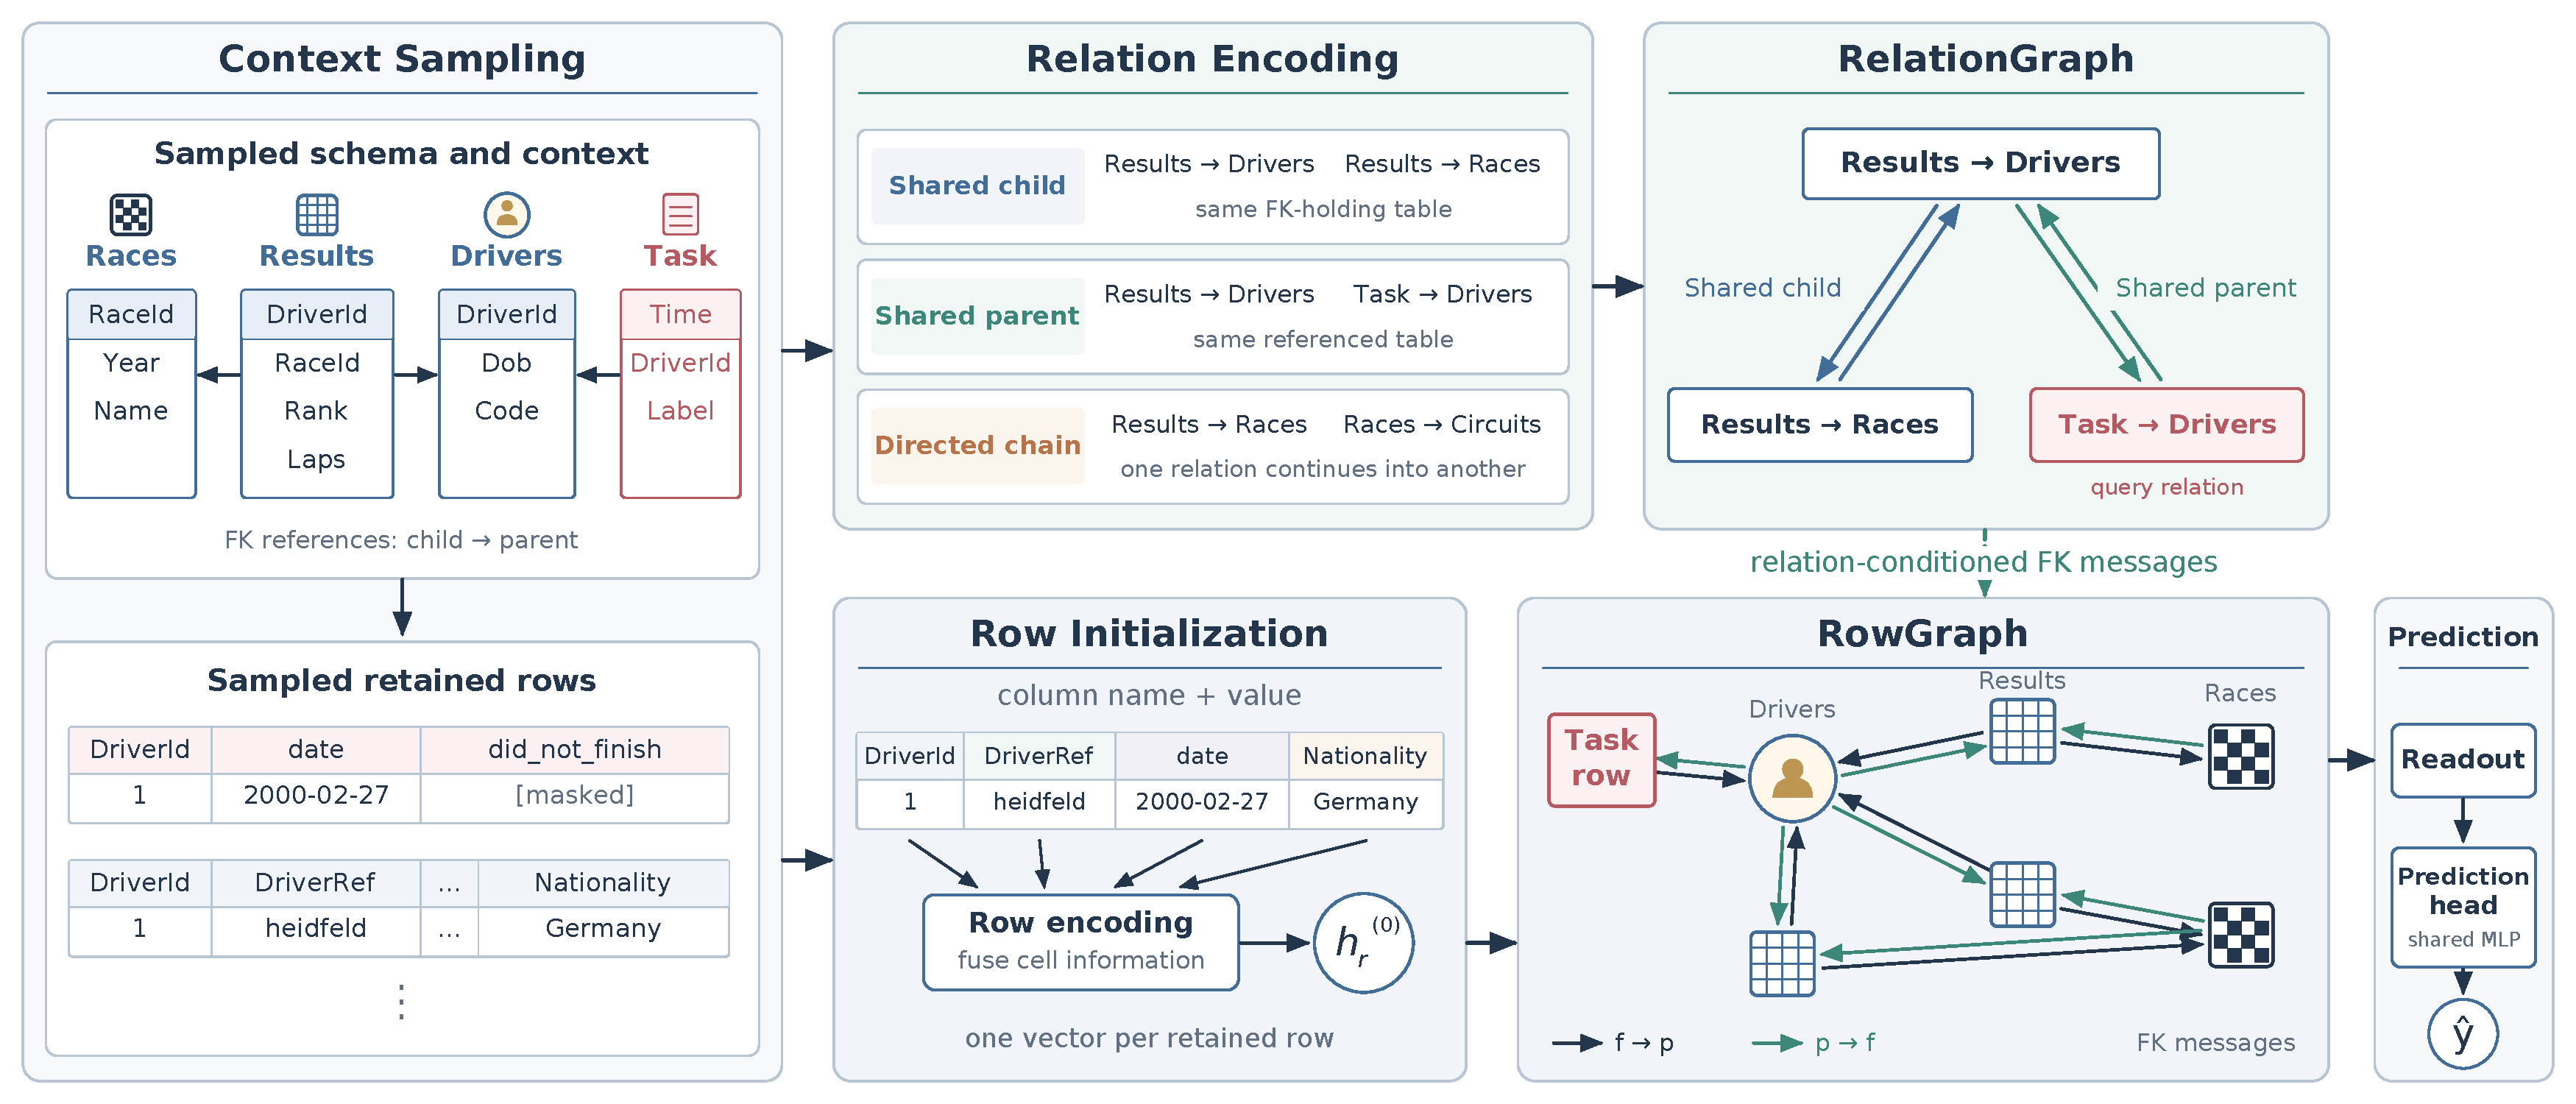
\includegraphics[width=\textwidth]{figures/architecture.pdf}
%   \caption{High-level overview of \model{}.  A bounded temporal context is
%   sampled, and visible heterogeneous cells are pooled once into row states.
%   The retained PK--FK links instantiate two coupled graphs: an instance-level
%   bidirectional row graph and a query-conditioned relation graph over ordered
%   child--parent table pairs.  The relation states condition the corresponding
%   foreign-to-primary ($\fkp$) and primary-to-foreign ($\pkf$) row messages,
%   after which a shared candidate scorer, abstracted by the MLP block, produces
%   the prediction.  Candidate nodes and label edges are omitted for clarity;
%   red marks the query table, row, and seeded relation.}
%   \label{fig:architecture}
% \end{figure*}

% These representations guide how information propagates between records;
% prediction further requires integrating record contents and task context.
% We therefore introduce \model{} (Figure~\ref{fig:architecture}), which
% couples RelationGraph with a row-level reasoning and candidate-prediction
% architecture. Within a bounded, temporally filtered context, shared encoders
% aggregate heterogeneous cell values into row representations, and retained
% PK--FK links connect these rows into a graph. The inferred relation
% representations condition bidirectional messages, guiding multi-hop
% aggregation of evidence across records. To incorporate historical task
% labels, we further augment the graph with two shared class-candidate nodes
% representing False and True. These nodes aggregate messages from context rows
% with matching labels, and a shared scorer compares the query row with each
% candidate to produce the prediction. Together, these components combine
% transferable relation representations, compact row-level reasoning, and
% context-aware prediction using parameters shared across databases and tasks.

% Our contributions are:
% \begin{itemize}
%   \item We introduce a query-conditioned RelationGraph to construct
%   transferable relation representations.
%   \item We combine relation-guided RowGraph reasoning with shared True/False
%   candidate nodes for prediction across databases.
%   \item We evaluate \model{} on ten binary RelBench tasks, comparing its
% accuracy and parameter efficiency with baselines, examining the effect of
% model size, and analyzing which information the trained model relies on.

% \end{itemize}


% \section{Introduction}
% \label{sec:introduction}

% Relational databases support predictive decisions in commerce, finance,
% science, and online platforms. The evidence for a prediction is usually
% spread over linked tables: whether a Formula~1 driver will fail to finish the
% next race depends on the driver's earlier results, the races in which they
% were obtained, and the other drivers in those races. Relational Deep Learning
% (RDL) represents rows as nodes and primary--foreign key (PK--FK) references as
% edges, and learns to aggregate this evidence with graph neural networks (GNNs)
% \citep{fey2024rdl}; RelBench provides real-world databases and temporal
% prediction tasks for this setting \citep{robinson2024relbench}. These models,
% however, are trained for one database and one task, so every new database or
% prediction target requires another cycle of training and validation.
% Cross-dataset entity classification removes this cycle: a model trained on a
% collection of databases predicts entity labels in an unseen database without
% updating its parameters.

% Relational foundation models have made this setting feasible
% \citep{ranjan2026rt,ranjan2026rtj,kothapalli2026plurel,hudovernik2026kumorfm2}.
% To cope with databases whose tables and columns differ, they represent a
% database as generic units, such as cells in \RT{} \citep{ranjan2026rt} or rows
% and sampled examples in KumoRFM-2 \citep{hudovernik2026kumorfm2}, and use
% attention to learn from data which of these units are relevant to a
% prediction; RDBLearn similarly relies on a tabular in-context learner that
% attends over thousands of labeled examples \citep{xu2026rdblearn}. Much of
% what this attention has to discover is, however, structural. \RT{}'s own
% analysis attributes its zero-shot transfer to task context, relational
% attention patterns, and schema semantics \citep{ranjan2026rt}; the first two
% amount to knowing which records carry labels and which records are linked.
% A database states this information explicitly: PK--FK references identify
% linked records, the schema specifies how tables are connected, and the task
% table and timestamps provide the label history and its temporal order.
% Learning it through attention costs model capacity and computation; \RT{},
% for example, uses 22M parameters and attends over cell-level tokens in every
% layer.

% GNNs take the opposite approach. Their aggregation follows PK--FK edges
% directly, which makes them compact, but they distinguish structure through
% parameters tied to one schema: an encoder for each table, a weight matrix for
% each relation, and an output head for each task
% \citep{fey2024rdl,chen2025relgnn}. These parameters make structural
% distinctions explicit. In Formula~1, \texttt{Results}$\rightarrow$\texttt{Drivers}
% and \texttt{Results}$\rightarrow$\texttt{Races} are both child-to-parent links,
% but the first connects a result to the driver who obtained it and the second
% to the race in which it occurred; a relation-specific weight lets the model
% treat the two kinds of evidence differently. In an unseen database none of
% these parameters is defined. Griffin shares its encoders across databases, but
% aggregates cells with attention and is fine-tuned for each downstream task
% \citep{wang2025griffin}. Simply removing relation-specific weights makes a GNN
% transferable but discards the distinctions they encode, since messages along
% all PK--FK links are then processed alike. On F1 driver-DNF, for instance,
% retraining our model without its relation representations lowers AUROC from
% 81.2 to 74.2 (Section~\ref{sec:result}).
% % TODO: add the retrained ablation (results/ablation/retrained) to Section 5;
% % the numbers above are seed 2 and predate the relation-key fix.

% The central challenge is therefore to retain the efficiency of
% structure-following aggregation while expressing these structural distinctions
% without parameters specific to any database. Meeting it makes prediction on an
% unseen database direct, because the database structure rather than learned
% attention specifies which records are related and how, and efficient, because
% no capacity is spent on recovering this structure from data.

% \begin{figure*}[t]
%   \centering
%   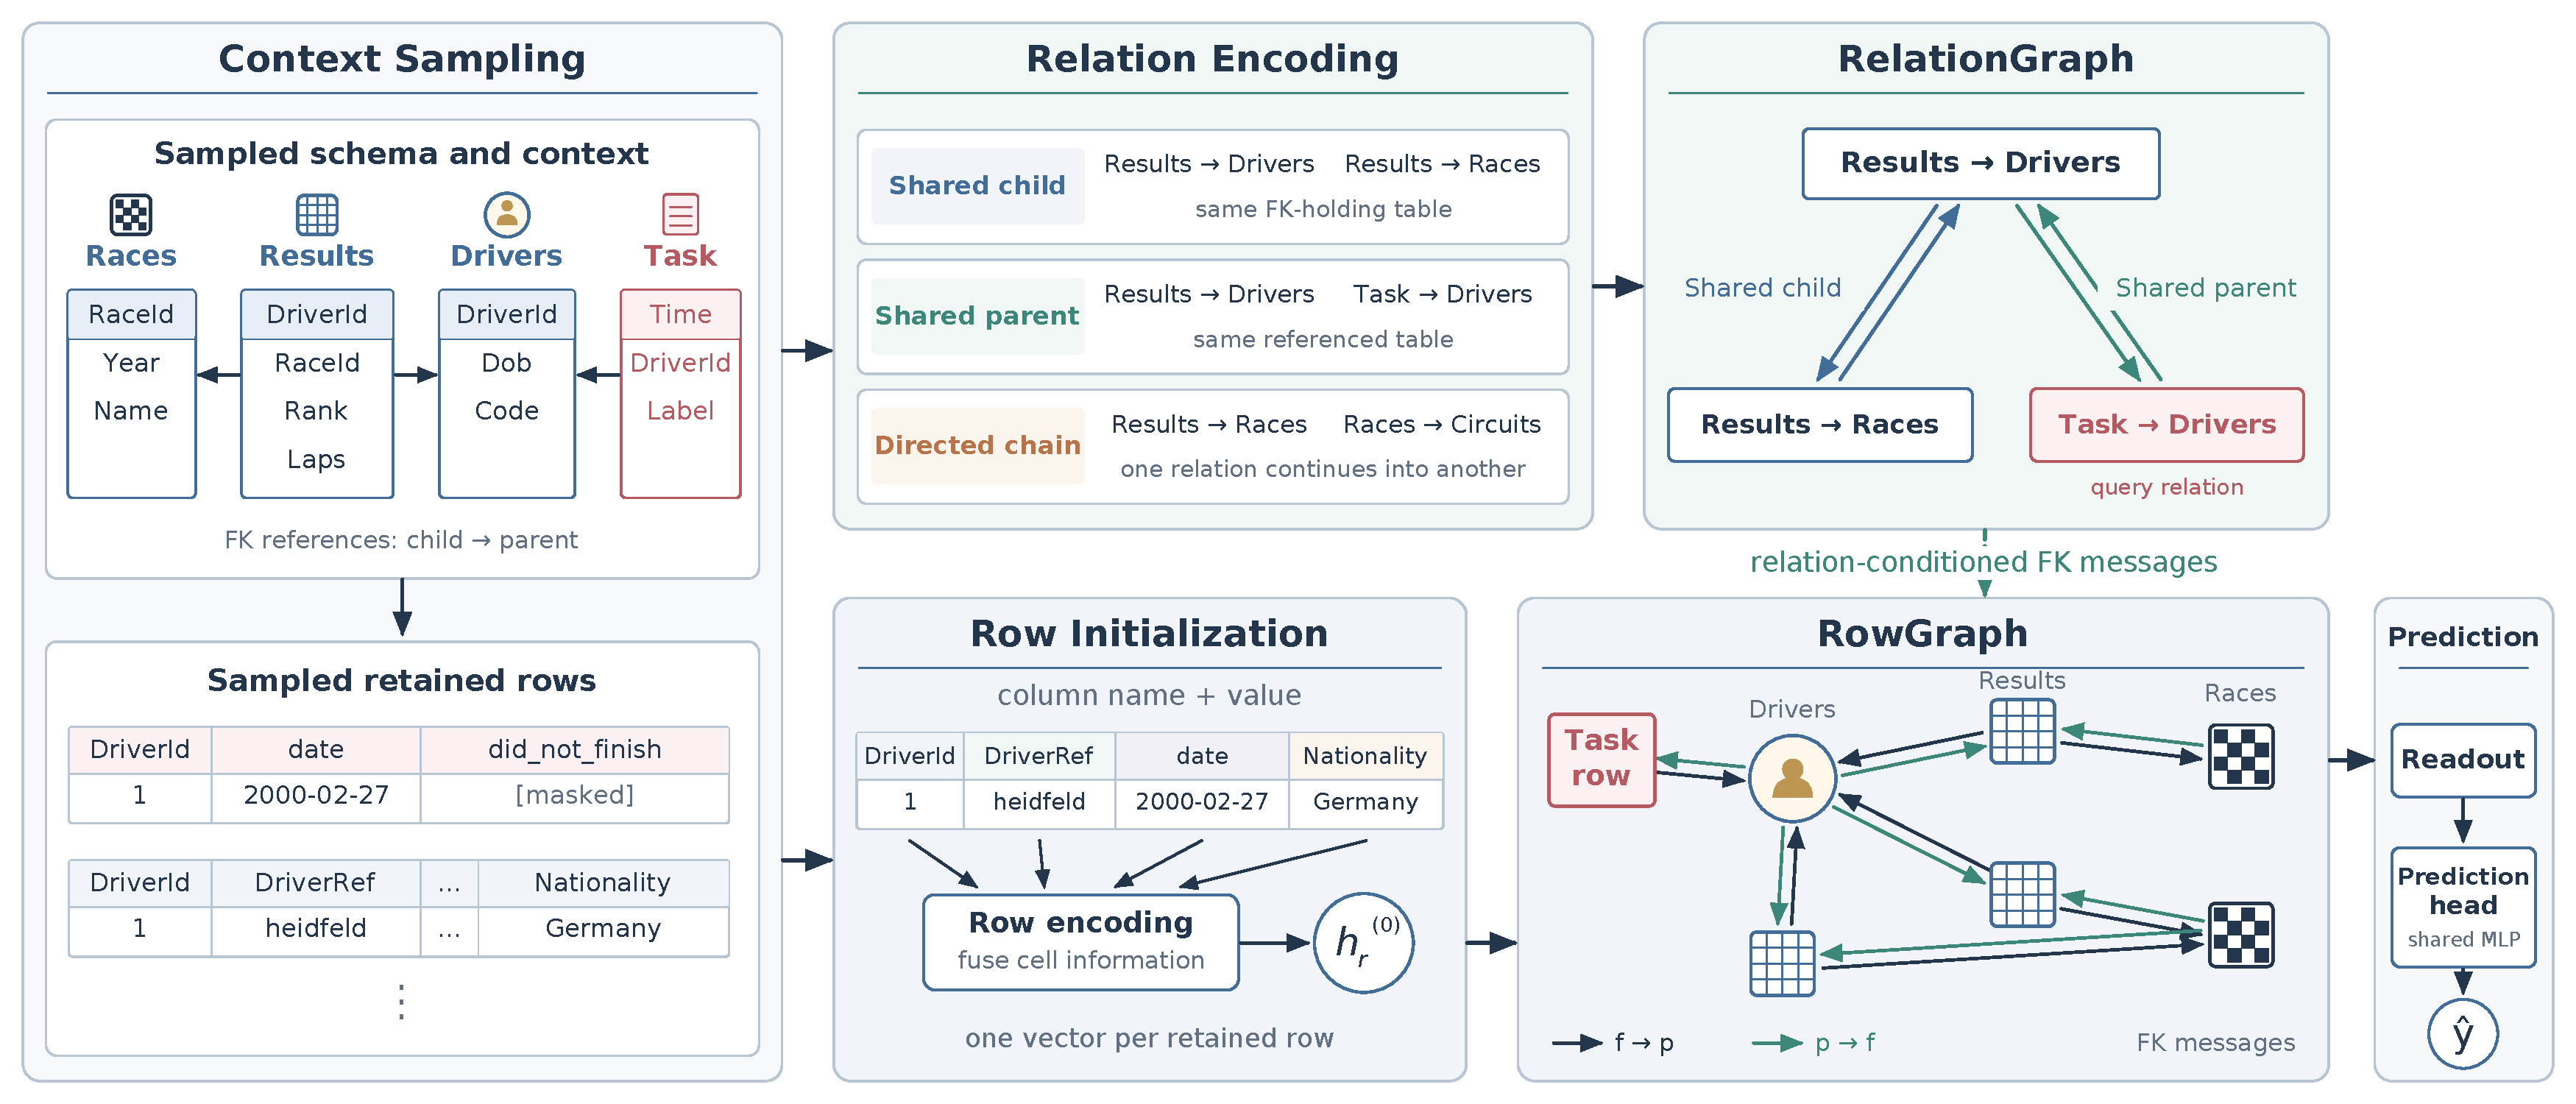
\includegraphics[width=\textwidth]{figures/architecture.pdf}
%   \caption{High-level overview of \model{}.  A bounded temporal context is
%   sampled, and visible heterogeneous cells are pooled once into row states.
%   The retained PK--FK links instantiate two coupled graphs: an instance-level
%   bidirectional row graph and a query-conditioned relation graph over ordered
%   child--parent table pairs.  The relation states condition the corresponding
%   foreign-to-primary ($\fkp$) and primary-to-foreign ($\pkf$) row messages,
%   after which a shared candidate scorer, abstracted by the MLP block, produces
%   the prediction.  Candidate nodes and label edges are omitted for clarity;
%   red marks the query table, row, and seeded relation.}
%   \label{fig:architecture}
% \end{figure*}

% We address this challenge with \model{} (Figure~\ref{fig:architecture}), a
% lightweight GNN whose parameters are tied only to roles that every database
% shares. Each distinction above can be derived from structure present in any
% database. \emph{Linked records} follow from PK--FK references: as in \RT{},
% cells are encoded from their values and column names with encoders shared
% across tables; \model{} pools them once into one vector per record and passes
% messages along PK--FK links with two edge types, child-to-parent and
% parent-to-child, that are common to all databases. \emph{The role of a
% relation} follows from how it shares tables with other relations: adapting
% the relation graph of knowledge-graph foundation models
% \citep{lee2023ingram,galkin2024ultra}, \model{} treats each child--parent
% table pair as a relation, connects relations that share a table, and
% propagates from the relation of the query to derive representations that
% condition the messages along each relation. \emph{Labels} follow from the
% task table: records with known labels are connected to one node per class,
% and the query is scored against these nodes, so no task-specific output layer
% is needed; each timestamped record also carries its time relative to the
% prediction. Because the database structure, rather than learned attention,
% determines how information is aggregated, all computation after cell encoding
% scales with the number of records and links rather than cells.

% On ten binary classification tasks from RelBench under leave-database-out
% transfer, \model{} reaches \mainAUROC{} macro AUROC with \mainParams{}
% parameters, on par with the strongest baseline, which uses about eight times as
% many parameters, and its accuracy grows with width to \wideAUROC{} at
% \wideParams{} parameters (Section~\ref{sec:standard_results}). Our analysis
% shows that two-hop neighborhoods suffice and that the entity's own label
% history is the dominant signal (Section~\ref{sec:case_study}).

% Our contributions are:
% \begin{itemize}
%   \item We identify the schema-specific parameters through which relational
%   GNNs encode structure and propose \model{}, a row-level GNN that replaces
%   them with counterparts shared across databases, so that the database
%   structure, rather than learned attention, determines how information is
%   aggregated.
%   \item We adapt the relation graph of knowledge-graph foundation models to
%   relational databases, defining relations as child--parent table pairs and
%   using the resulting representations to condition message passing between
%   records, so that relations in unseen schemas are distinguished without
%   relation-specific parameters.
%   \item We evaluate \model{} on ten RelBench tasks under leave-database-out
%   transfer, showing that with \mainParams{} parameters it performs on par with
%   or better than attention-based baselines about eight times its size, and
%   analyze which information it relies on.
% \end{itemize}

\section{Introduction}
\label{sec:introduction}

Relational databases support predictive decisions in commerce, finance,
science, and online platforms. The evidence for a prediction is usually
spread over linked tables: whether a Formula~1 driver will fail to finish the
next race depends on the driver's earlier results, the races in which they
were obtained, and the other drivers in those races. Relational Deep Learning
(RDL) represents rows as nodes and primary--foreign key (PK--FK) references as
edges, and learns to aggregate this evidence with graph neural networks (GNNs)
\citep{fey2024rdl}; RelBench provides real-world databases and temporal
prediction tasks for this setting \citep{robinson2024relbench}. These models,
however, are trained for one database and one task, so every new database or
prediction target requires another cycle of training and validation.
Cross-dataset entity classification removes this cycle: a model trained on a
collection of databases predicts entity labels in an unseen database without
updating its parameters.

Relational foundation models have made this setting feasible
\citep{ranjan2026rt,ranjan2026rtj,kothapalli2026plurel,hudovernik2026kumorfm2}.
To cope with databases whose tables and columns differ, they represent a
database as generic units, such as cells in \RT{} \citep{ranjan2026rt} or rows
and sampled examples in KumoRFM-2 \citep{hudovernik2026kumorfm2}, and use
attention to learn from data which of these units are relevant to a
prediction; RDBLearn similarly relies on a tabular in-context learner that
attends over thousands of labeled examples \citep{xu2026rdblearn}. Much of
what this attention has to discover is, however, structural. \RT{}'s own
analysis attributes its zero-shot transfer to task context, relational
attention patterns, and schema semantics \citep{ranjan2026rt}; the first two
amount to knowing which records carry labels and which records are linked.
A database states this information explicitly: PK--FK references identify
linked records, the schema specifies how tables are connected, and the task
table and timestamps provide the label history and its temporal order.
Learning it through attention costs model capacity and computation; \RT{},
for example, uses 22M parameters and attends over cell-level tokens in every
layer.

GNNs take the opposite approach. Their aggregation follows PK--FK edges
directly, which makes them compact, but they distinguish structure through
parameters tied to one schema: an encoder for each table, a weight matrix for
each relation, and an output head for each task
\citep{fey2024rdl,chen2025relgnn}. These parameters make structural
distinctions explicit. In Formula~1, \texttt{Results}$\rightarrow$\texttt{Drivers}
and \texttt{Results}$\rightarrow$\texttt{Races} are both child-to-parent links,
but the first connects a result to the driver who obtained it and the second
to the race in which it occurred; a relation-specific weight lets the model
treat the two kinds of evidence differently. In an unseen database none of
these parameters is defined. Griffin shares its encoders across databases, but
aggregates cells with attention and is fine-tuned for each downstream task
\citep{wang2025griffin}. Simply removing relation-specific weights makes a GNN
transferable, but it then applies the same transformation to messages along
every PK--FK link, so the distinction has to be recovered from record content,
as attention-based models do from the table and column names attached to each
token \citep{ranjan2026rt}.
On F1 driver-DNF, for instance,
% retraining our model without its relation representations lowers AUROC from
% 81.2 to 74.2 (Section~\ref{sec:result}).

The central challenge is therefore to retain the efficiency of
structure-following aggregation while expressing these structural distinctions
without parameters specific to any database. Meeting it makes prediction on an
unseen database direct, because the database structure rather than learned
attention specifies which records are related and how, and efficient, because
no capacity is spent on recovering this structure from data.

\begin{figure*}[t]
  \centering
  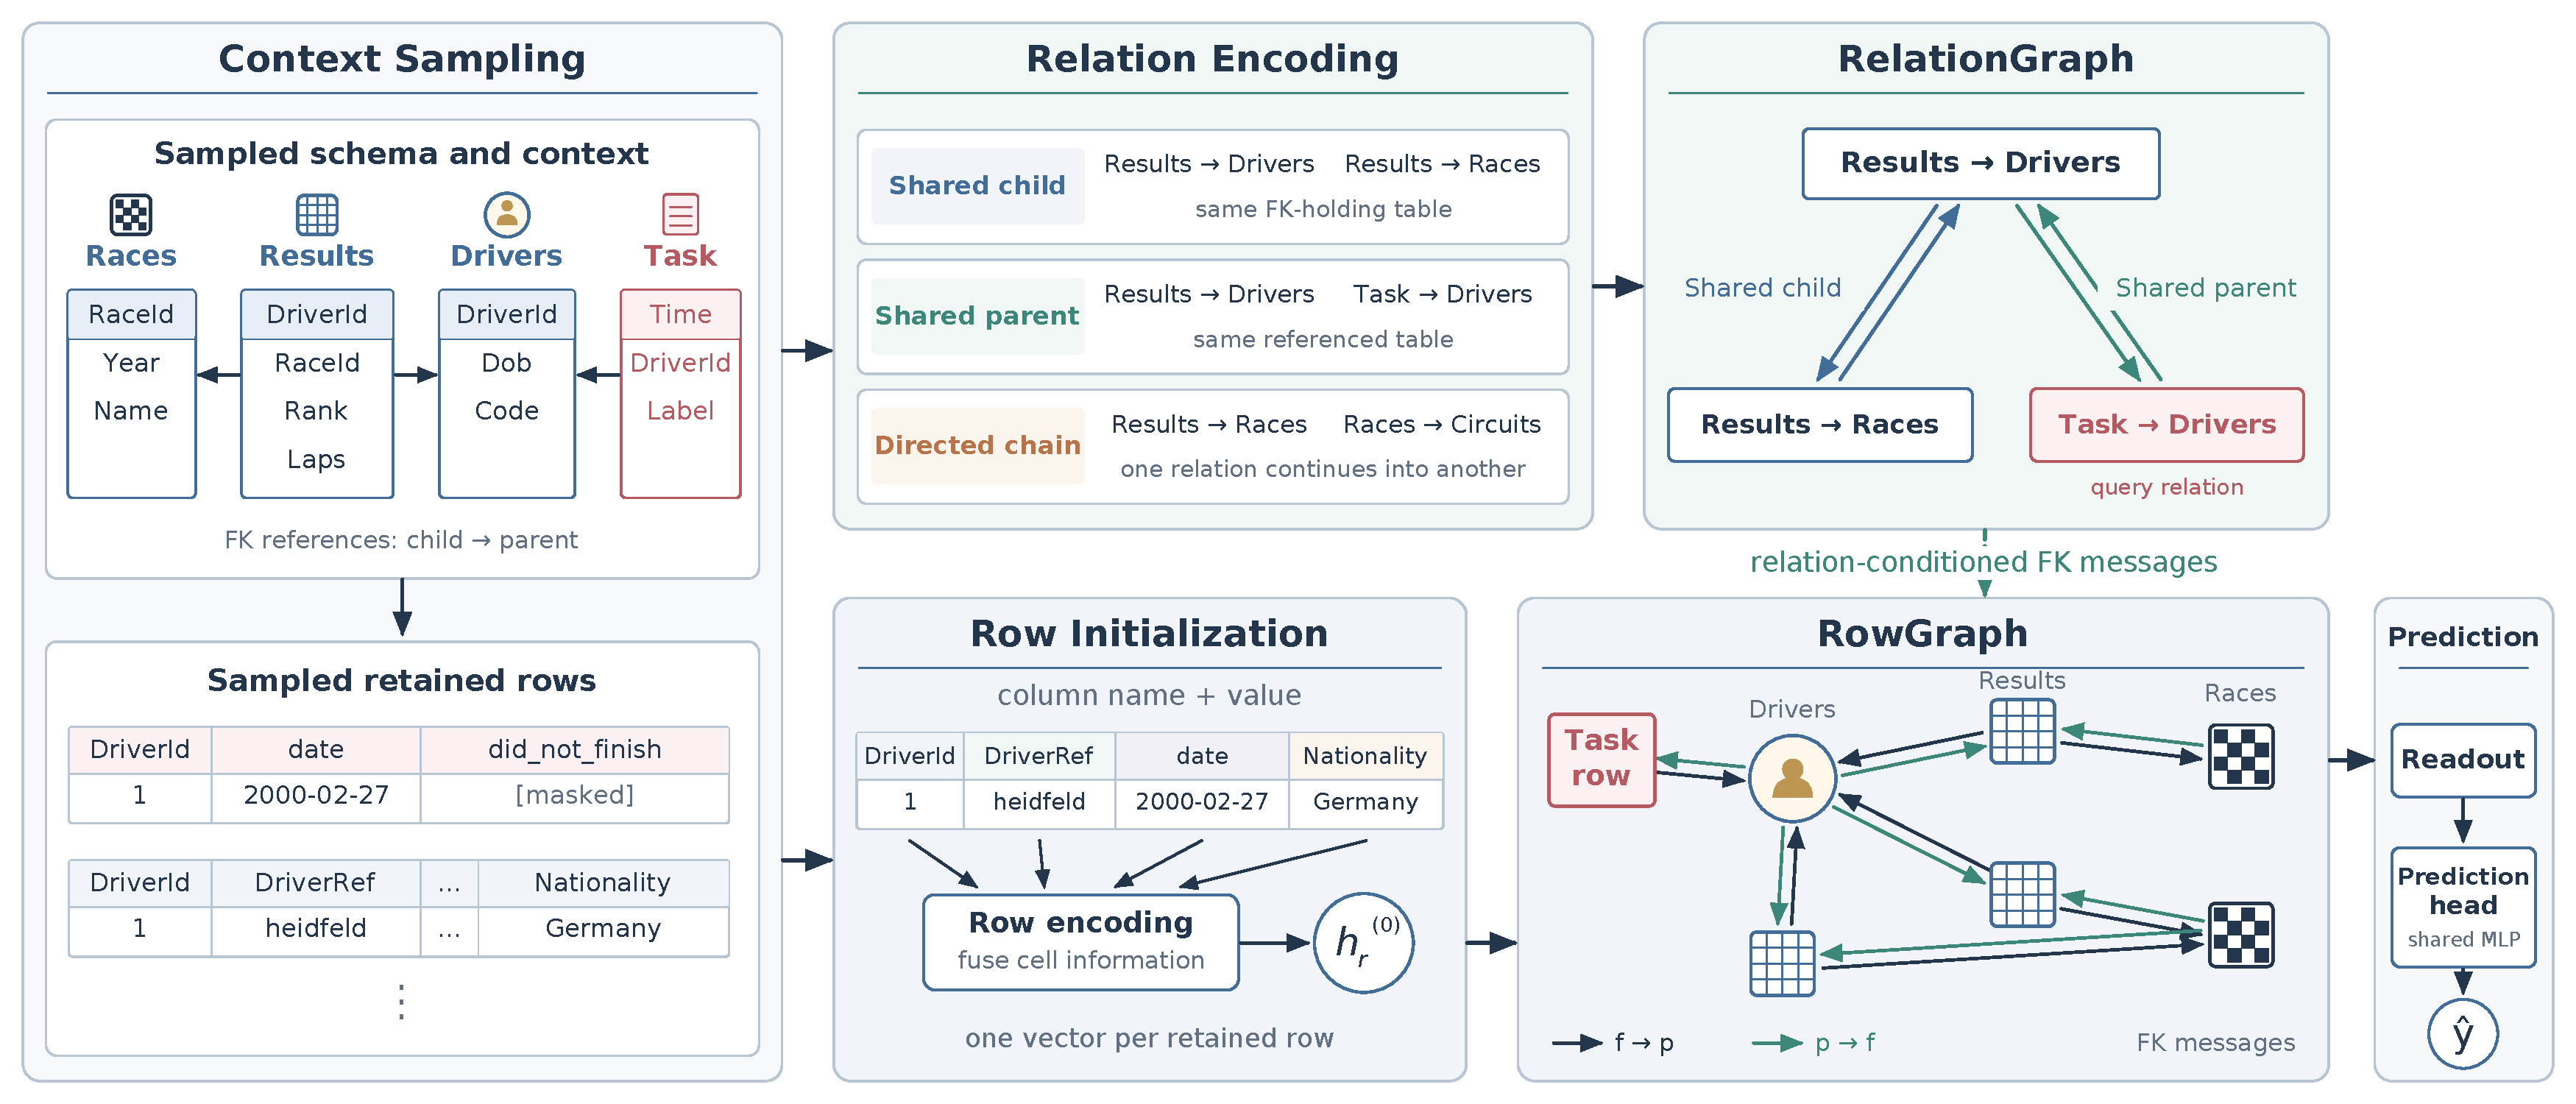
\includegraphics[width=\textwidth]{figures/architecture.pdf}
  \caption{Overview of \model{}. Context Sampling collects a bounded context
  around the query row that respects the prediction time: the tables and
  foreign-key references it contains (upper panel) and the sampled rows
  (lower panel). Row Initialization encodes the cells of each row into one
  vector. Relation Encoding links the foreign-key relations that share a
  table, and RelationGraph computes one representation per relation,
  conditioned on the query relation. These representations condition the
  child-to-parent (f$\rightarrow$p) and parent-to-child (p$\rightarrow$f)
  messages of RowGraph. Prediction compares the final state of the query row
  with class nodes that collect the labels of earlier task rows; the class
  nodes and their edges are omitted from the drawing. Red marks the query
  table, the query row, and the query relation.}
  \label{fig:architecture}
\end{figure*}

We address this challenge with \model{} (Figure~\ref{fig:architecture}), a
lightweight GNN whose parameters are tied only to roles that every database
shares. Each distinction above can be derived from structure present in any
database. \emph{Linked records} follow from PK--FK references: as in \RT{},
cells are encoded from their values and column names with encoders shared
across tables; \model{} pools them once into one vector per record and passes
messages along PK--FK links with two edge types, child-to-parent and
parent-to-child, that are common to all databases. \emph{The role of a
relation} follows from how it shares tables with other relations: adapting
the relation graphs that knowledge-graph models use to represent unseen
relations \citep{lee2023ingram,galkin2024ultra}, \model{} treats each child--parent
table pair as a relation, connects relations that share a table, and
propagates from the relation of the query to derive representations that
condition the messages along each relation. \emph{Labels} follow from the
task table: records with known labels are connected to one node per class,
and the query is scored against these nodes, so no task-specific output layer
is needed; each timestamped record also carries its time relative to the
prediction. Because the database structure, rather than learned attention,
determines how information is aggregated, all computation after cell encoding
scales with the number of records and links rather than cells.

On ten binary classification tasks from RelBench under leave-database-out
transfer, \model{} reaches \mainAUROC{} macro AUROC with \mainParams{}
parameters, on par with the strongest baseline, which uses about eight times as
many parameters, and its accuracy grows with width to \wideAUROC{} at
\wideParams{} parameters (Section~\ref{sec:standard_results}). Our analysis
shows that two-hop neighborhoods suffice and that the entity's own label
history is the dominant signal (Section~\ref{sec:case_study}).

Our contributions are:
\begin{itemize}
  \item We identify the schema-specific parameters through which relational
  GNNs encode structure and propose \model{}, a row-level GNN that replaces
  them with counterparts shared across databases, so that the database
  structure, rather than learned attention, determines how information is
  aggregated.
  \item We bring to relational databases the relation graphs that
  knowledge-graph models use to represent unseen relations, defining relations
  as child--parent table pairs and
  using the resulting representations to condition message passing between
  records, so that relations in unseen schemas are distinguished without
  relation-specific parameters.
  \item We evaluate \model{} on ten RelBench tasks under leave-database-out
  transfer, showing that with \mainParams{} parameters it performs on par with
  or better than attention-based baselines about eight times its size, and
  analyze which information it relies on.
\end{itemize}